\section{Variables of Interest}
\textbf{Predictor Variables} \\
As outlined in the previous section, all independent variables are standardized to z-scores. Based on our hypotheses, they are the z-scores of (1) daily sentiment; (2) fear, (3) trust, (4) joy and, finally, (5) anticipation all expressed on Twitter. Descriptive statistics for the 5 independent variables are detailed in Table 3.2 . All the z-score variables have an approximately 0 mean and a standard deviation of 1, closely following the characteristics of a normally distributed series. However, the sentiment index and anticipation series have a noticeable negative skew, implying that the series have positive sentiment and high anticipation on most days, but there are some outliers with very negative sentiment/low anticipation. Moreover, all the series are leptokurtic, meaning that they have heavy fat tails. And especially the trust series appears to have extreme outliers in its values. This is also evidenced in Figure 3.3. Trust levels skyrocketed in October 2020, at the time when multiple vaccines were successfully completing phases 2 and 3 of trials.
\begin{figure}[htp]
    \centering
    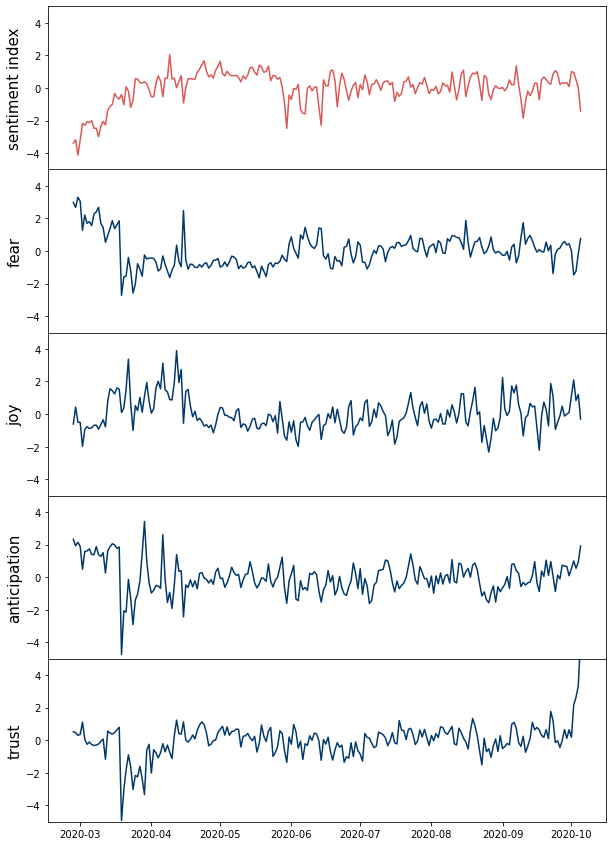
\includegraphics[width=12cm]{methods/Emotions.png}
    \caption{Z-scores of sentiment index and aggregate emotions.}
    \label{fig:Emotions}
\end{figure}

\begin{table}[h]
\centering
\caption{Descriptive statistics for independent variables.}
\vspace{0.5cm}
\begin{tabular}{lllll}
\hline\hline
Variable & Mean & SD & Skewness & Kurtosis \\ \hline
Sentiment index & 0.104 & 0.894 & -1.019 & 4.238 \\
Fear & -0.050 & 0.914 & 0.193 & 3.581 \\
Trust &  0.021 & 1.016 & 0.298 & 15.318 \\
Joy & -0.085 & 0.961 & 0.602 & 3.631 \\
Anticipation & -0.014 & 0.960 & -0.735 & 6.520 \\
\hline
\end{tabular}
\begin{tablenotes}
    \small
      \item{\textit{Note: The kurtosis metric outlines excess kurtosis, as opposed to the absolute kurtosis value.\\Hence, normal distribution would correspond to an excess kurtosis of zero}}
\end{tablenotes}
\end{table}

\textbf{Outcome Variable} \\
Our outcome of interest concerns the S\&P500 price series. When testing the properties of S\&P500 raw prices, we find evidence of unit root non-stationarity in the series (please see Table A.3 in the Appendix). This has no implications for the neural network model we are using, since neural networks do not pose any limitations on variable distributions. And we, therefore, use raw S\&P500 prices as outcome variable in the neural network models. 

On the other hand, the linear Granger causality method requires that the variables are unit root stationary \parencite{wooldridge2015introductory}. To overcome this issue and prevent any potential bias in the Granger causality results which unit root price series could introduce, we compute the day-to-day changes of the price series. This form of first differencing is outlined in Equation 3.2. By taking the day-to-day price changes, we eliminate any unit root non-stationarity (as evidenced in Table A.6). We, therefore, use day-to-day changes in S\&P500 prices as our dependent variable in the Granger causality model. 

\begin{ceqn}
\begin{align}
D_t={S\&P500}_t-{S\&P500}_{t-1}
\end{align}
\end{ceqn}

The descriptive statistics of the S\&P 500 prices and their day-to-day changes are outlined in Table 3.3. We see that the daily price changes are, on average, positive which suggests an overall rising price trend. The negative skew illustrates that despite the general positive trend, there are some very substantial price crashes in the series.

\begin{table}[h]
\centering
\caption{Descriptive statistics for dependent variable.}
\vspace{0.5cm}
\begin{tabular}{lllll}
\hline\hline
Variable & Mean & SD & Skewness & Kurtosis \\ \hline
Raw S\&P500 price & 3062.813 & 295.680 &  -0.635 & -0.277 \\
Day-to-day S\&P500 price difference & 2.989 & 72.871 &  -0.806 & 7.127 \\
\hline
\end{tabular}
\begin{tablenotes}
    \small
      \item{\textit{Note: The kurtosis metric outlines excess kurtosis, as opposed to the absolute kurtosis value. \\Hence, normal distribution would correspond to an excess kurtosis of zero}}
\end{tablenotes}
\end{table}

\section{Empirical Strategy}
\subsection{Linear Granger Causality}

We use linear Granger causality analysis to evaluate Hypotheses 1-5 as well as to provide partial evidence for Hypothesis 6. In general, Granger causality technique is based on the assumption that if a variable X causes variable Y, then changes in X will systematically
precede changes in Y. Therefore, lagged
values of X must be significantly correlation
with present values of Y. It must be pointed out, however, that correlation does not imply causation and we are not testing whether one time series causes the other, but merely whether one time series has predictive information about the other.

We run two types of linear models to test our hypotheses: 
(1) an autoregressive model of past changes in S&P 500 prices, outlined in Equation 3.3; 
(2) an autoregressive model which additionally incorporates one of the four different emotions or the unidimensional Twitter sentiment index, outlined in Equation 3.4.\\
\begin{ceqn}
\begin{align}
L_1:D_t = \alpha + \sum_{i=1}^{n}{\beta_iD_{t-i} + \epsilon_t}\\ 
L_2:D_t = \alpha + \sum_{i=1}^{n}{\beta_iD_{t-i} + \sum_{i=1}^{n}{\delta_iX_{t-i}} + \epsilon_t} 
\end{align}
\end{ceqn}

The variable X in Model (2) represents either: (a) sentiment index, (b) fear, (c) joy, (d) trust, or (e) anticipation. Model (1) and Model (2) are nested Auto Regressive Distributed Lag models. The nested structure allows us to conduct likelihood ratio F-tests. More specifically, we are testing whether the specific emotions, or the unidimensional Twitter index expressed in variable X have predictive content for S&P500 above and beyond that contained in past changes of S&P 500 prices \parencite{kirchgassner2012introduction}. 

Granger causality test statistics are very sensitive to the lag length chosen for the underlying VAR model and too high selected number of lags (i.e. overfitting) increases the probability of false positive results \parencite{bruns2019lag}. Therefore, we choose the exact lag length prior to testing. Given that previous research by \textcite{bollen2011twitter} incorporated 1-7 lags in their linear model specifications and found that some emotions Granger cause DJIA values for up to 6 days worth of lags, we also consider up to 6 day-lags for the Granger causality analysis. But out of the potential 1-6 day lag specifications, we only select the one lag specification that minimises both the AIC \parencite{akaike1974new} and BIC \parencite{schwarz1978estimating} prior to analysis. In case that AIC and BIC yield different results, we use the model which minimises AIC - as recommended by \textcite{thornton1985lag}, \textcite{ozcicek1999lag}. To illustrate, in a Monte Carlo simulation study by \textcite{ozcicek1999lag}, the AIC criterion selects the true lags more frequently than BIC, and also more often than all other considered criteria in symmetric VAR models. 


\subsection{Fully Connected Neural Network}

To address non-linear effects that are indisputably present in the actual data-generating process, and to evaluate Hypothesis 6, we use fully connected neural network models. Our decision to use fully connected networks, rather than Self-Organizing Fuzzy neural networks, as was performed in \textcite{bollen2011twitter}, has its empirical grounding. Since the publishing of Bollen et al. paper, the non-linear modelling literature has diverted away from fuzzy logic towards modern neural networks, which require fewer assumptions prior to the main analysis. Put differently, fewer parameters must be explicitly pre-specified in fully connected neural network models relative to fuzzy neural networks, which prevents the potentiality of incorrect assumption setting \parencite{goodfellow2016deep}. 

Moreover, other neural network models besides fully connected neural networks are being increasingly applied to stock market prediction, including long short-term memory networks and convolutional neural networks  \parencite{fischer2018deep, chen2018stock}. However, both long short-term memory networks and convolutional neural network models have a well-known tendency to overfit small datasets by memorizing inputs rather than training, which leaves them arguably not well-suited for our analysis of small scale dataset \parencite{hochreiter1997lstm, lecun1989backpropagation}. 

We run 2 fully connected neural network models - (1) model that takes as inputs only past values of S\&P500 prices, and (2) model that takes as inputs S\&P500 prices, emotions and sentiment of the past days. To predict the S\&P500 value on day t, the inputs of our fully connected neural network (2) include lagged values of S\&P500 prices, emotions and the overall sentiment of the past n days. The selected number of incorporated lags - n, is determined through the process of hyper-parameter tuning \parencite{claesen2015hyperparameter}. This tuning procedure selects the best non-linear naive/baseline model (i.e., model with just S\&P500 prices) that we can obtain given our sample size constraints. In consequence, the tuning procedure ensures that the goodness-of-fit comparison between our baseline model and the model that additionally includes emotions and sentiment is fair and does not inflate our contribution.

The sentiment and emotion inputs are linearly scaled to [0,1], in order to ensure that the mood inputs have similar initial weights in the model. However, since we are interested in our outcome variable of S\&P500 prices, we do not linearly scale the S\&P500 price values prior to analysis. This, in consequence, determines the selection of our activation function. The standard ReLU activation function works best when all input variables are linearly scaled. Since we do not linearly scale the lagged prices in our model, we instead use the Leaky ReLU activation function, which is well-suited for negative input values \parencite{nwankpa2018activation}. The Leaky ReLU function is detailed in Appendix Figure A.1.
 
Our fully connected neural network model has 3 layers. The decision to choose 3 layers stems from our limited sample size on one hand and the need to have at least 1 inner layer on the other hand. By choosing the relatively low number of layers, we are limiting the risk of model overfitting, while also ensuring that we provide some opportunity for the model to learn.

In mathematical terms, given that $\sigma$ is the Leaky Relu function, $x$ being the input, $a$ being the desired output,$M_1$, $M_2$, $M_3$, $b_1$, $b_2$, $b_3$ being the trainable parameters for the neural network and $L$ being the error, we obtain that our neural network can be expressed as: 

\begin{ceqn}
\begin{align}
y_1 = \sigma(\mathbf{M_1} * x + b_1) \\
y_2 = \sigma(\mathbf{M_2} * y_1 + b_2) \\
y = \sigma(\mathbf{M_3} * y_2 + b_3) \\
L = (a - y)^2
\end{align}
\end{ceqn}

Having calculated the loss for a given input and desired output, given $\alpha$ being the learning rate, we then update the trainable parameters using a variation of the following expression:

\begin{ceqn}
\begin{align}
M_n^{new} = M_n^{old} - \alpha\frac{\partial L}{\partial M_n^{old}} \\
b_n^{new} = b_n^{old} - \alpha\frac{\partial L}{\partial b_n^{old}} \\
\end{align}
\end{ceqn}

Given our small sample size, we divide the sample into a training set and a testing set by using a k-Fold Cross-Validation, rather than pre-specified training and testing periods. Guided by past research, we select 10 folds (k=10) in our k-Fold Cross-Validation procedure. According to \textcite{james2013introduction}, k=10 provides a good compromise between computational cost and bias of model performance estimates. Forecasting accuracy is then measured in terms of the average Mean Absolute Percentage Error (MAPE) and the direction accuracy (up or down) during the test period selected via k-Fold Cross-Validation procedure. The choice of MAPE and direction accuracy as key performance indicators was driven by past research (e.g. \textcite{bollen2011twitter}).
